\documentclass[11pt, a4paper]{article}
\usepackage[utf8]{inputenc}
\usepackage[T1]{fontenc}
\usepackage{amsmath}
\usepackage{amsfonts}
\usepackage{amssymb}
\usepackage{graphicx}
\usepackage{geometry}
\usepackage{hyperref}
\usepackage{listings} 
\usepackage{array}
\usepackage{longtable} 
\usepackage{float} 
\usepackage{enumitem} 
\usepackage{titling}

\geometry{a4paper, margin=1in}

\hypersetup{
    colorlinks=true,
    linkcolor=blue,
    filecolor=magenta,
    urlcolor=cyan,
    pdftitle={README - Proiect PCLP3 Partea I},
    pdfpagemode=FullScreen,
}

\lstdefinestyle{mystyle}{
    backgroundcolor=\color{lightgray!20},
    commentstyle=\color{green!50!black},
    keywordstyle=\color{blue},
    numberstyle=\tiny\color{gray},
    stringstyle=\color{purple},
    basicstyle=\ttfamily\footnotesize,
    breakatwhitespace=false,
    breaklines=true,
    captionpos=b,
    keepspaces=true,
    numbers=left,
    numbersep=5pt,
    showspaces=false,
    showstringspaces=false,
    showtabs=false,
    tabsize=2
}
\lstset{style=mystyle}

\newcommand{\studentname}{Rusu Andrei Ionut C2 341}
\title{Proiect PCLP3 - Partea I }
\date{\today}

% Redefine \maketitle to include student info at the top
\makeatletter
\renewcommand{\maketitle}{
  \begin{center}
    \Large \studentname \\
    \Huge \@title \\[1.5em]
    \large \@date
    \vspace{2em}
  \end{center}
  \par
  \thispagestyle{empty}
}
\makeatother

\begin{document}
\maketitle
\thispagestyle{empty}
\clearpage
\pagenumbering{arabic}

\section{Setul de Date}

Pentru aceasta tema am ales setul de date \href{https://www.kaggle.com/datasets/efeyldz/plant-communication-dataset-classification?resource=download}{Plant Communication Dataset} (pare sa fie generat sintetic) de pe platforma Kaggle, pentru o problema de clasificare.

Setul de date initial a fost augmentat prin adaugarea a trei noi coloane:
\sloppy
\begin{itemize}
    \item  \textbf{Soil\_Nutrient\_Level}: O coloana pentru nivelul de nutrienti din sol. Valorile au fost generate dintr-o distributie normala, cu medii si deviatii standard specifice fiecarui tip de mesaj (\texttt{Plant\_Message\_Type}), pentru a reflecta o legatura intre starea plantei si nutrienti - am folosit deviatii standard mari a.i. plajele de valori sa se intercaleze mult, pentru a nu crea o coloana puternic corelata cu coloana target.
    \item \textbf{Temperature\_Stress\_Factor}: O coloana categorica ('Low', 'Medium', 'High') derivata din \texttt{Ambient\_Temperature\_C}, indicand nivelul de stres termic.
    \item \textbf{Photosynthetic\_Efficiency\_Index}: Un indice calculat pe baza factorilor de stres termic, umiditate, nutrienti si expunere la soare, reflectand eficienta fotosintetica.
\end{itemize}

\subsection{Introducerea Zgomotului}
S-a adaugat zgomot la coloanele numerice relevante. Acest zgomot a fost generat dintr-o distributie normala cu media 0 si o deviatie standard egala cu 2\% din deviatia standard a fiecarei coloane. Coloanele afectate includ cele initiale numerice si cele nou create (\texttt{Soil\_Nutrient\_Level}, \  \texttt{Photosynthetic\_Efficiency\_Index}). Valorile au fost ulterior limitate pentru a ramane in intervale plauzibile.

\subsection{Simularea Valorilor Lipsa (NaN)}
\sloppy
S-au introdus valori NaN in mod aleatoriu pentru 5\% din instante in urmatoarele coloane: \texttt{Pollen\_Scent\_Complexity},\ \texttt{Bioluminescence\_Intensity\_Lux},\ \texttt{Growth\_Rate\_mm\_day},\ \texttt{Soil\_Nutrient\_Level},\ si \texttt{Soil\_Moisture\_Level}.

\section{Analiza Exploratorie a Datelor (EDA)}

\subsection{Sumarizare Generala a Setului de Date}
Initial, s-a realizat o sumarizare generala a setului de date, care a inclus:
\begin{itemize}[noitemsep, topsep=1pt]
    \item Dimensiunea setului de date: (1000 de randuri, 14 coloane).
    \item Tipurile de date pentru fiecare coloana: majoritatea float64, una int64 (\texttt{Symbiotic\_Fungus\_Present}) si doua de tip object (\texttt{Plant\_Message\_Type}, \texttt{Temperature\_Stress\_Factor}) (intial si Plant_ID, dar am scos o din setul de date dupa EDA, nefiind relevanta).
    \item Numarul de valori lipsa per coloana (inainte de imputare): 80 de valori lipsa pentru fiecare din cele 5 coloane mentionate anterior.
    \item Numarul de randuri duplicate: 0.
\end{itemize}

\subsection{Analiza Variabilelor Numerice}
Pentru variabilele numerice, s-au calculat statistici descriptive (medie, deviatie standard, min, max, quartile) si s-au generat boxplot-uri pentru a vizualiza distributiile si a identifica potentiali outlieri. Din boxploturi nu am identficat coloane cu valori aberante, ci mai degraba coloane cu plaje largi de valori. Totusi, am aplicat ulterior un tratament al outlierilor prin metoda IQR capping cu intervalele quantile 0.1/0.9.

\begin{figure}[H]
    \centering
    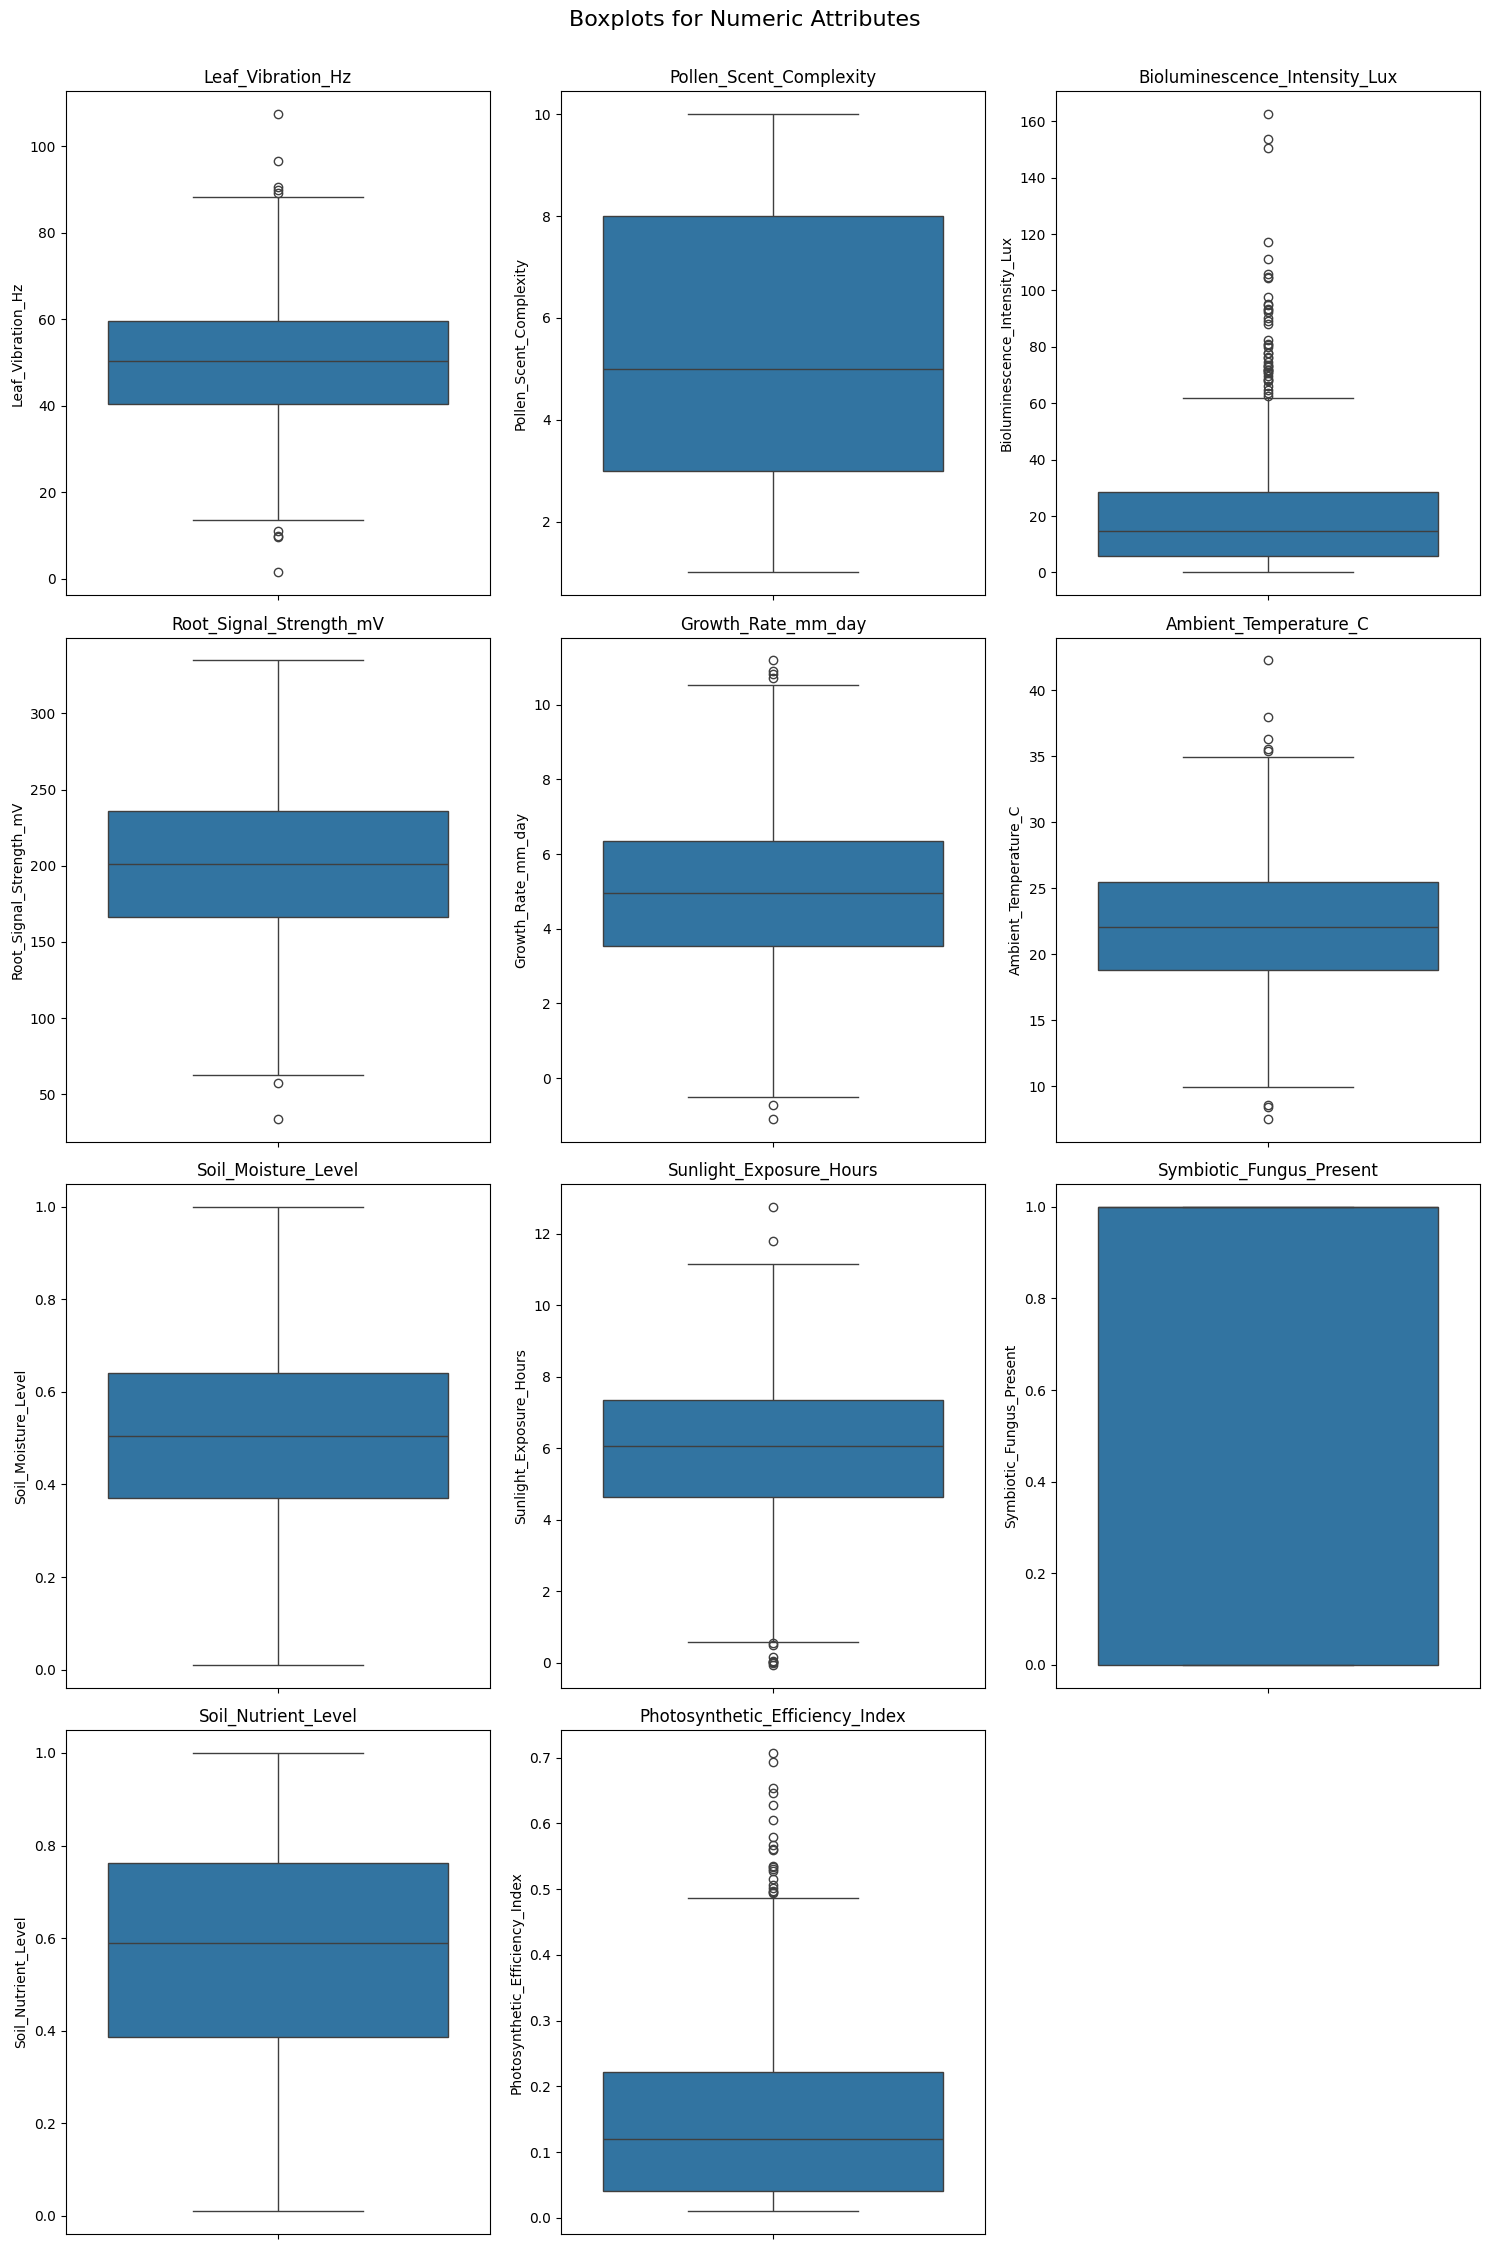
\includegraphics[width=0.9\textwidth]{numeric_boxplots.png}
    \caption{Boxplots date numerice}
    \label{fig:boxplots_numeric}
\end{figure}

\textit{Observatii:}
\begin{itemize}[noitemsep, topsep=1pt]
    \item \texttt{Leaf\_Vibration\_Hz}: Distributie relativ simetrica in jurul valorii de 50 Hz.
    \item \texttt{Pollen\_Scent\_Complexity}: Valori intre 1 si 10, cu mediana la 5.
    \item \texttt{Bioluminescence\_Intensity\_Lux}: O distributie puternic asimetrica la dreapta, cu multe valori mici si cativa posibili outlieri semnificativi cu valori mari.
    \item \texttt{Photosynthetic\_Efficiency\_Index}: Majoritatea valorilor sunt concentrate in jumatatea inferioara a intervalului [0,1].
\end{itemize}

\subsection{Analiza Variabilelor Categorice}
Pentru variabilele categorice (\texttt{Plant\_Message\_Type} si \texttt{Temperature\_Stress\_Factor}), s-au analizat numarul de valori unice si distributia acestora prin countplot-uri.

\begin{figure}[H]
    \centering
    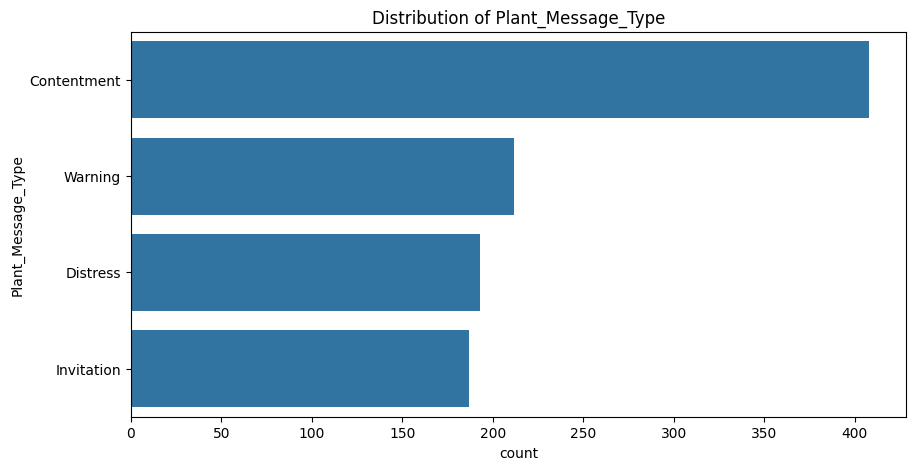
\includegraphics[width=\linewidth]{message_distr.png}
    \caption{Distributia \texttt{Plant\_Message\_Type}.}
    \label{fig:countplot_message}
\end{figure}

\begin{figure}[H]
    \centering
    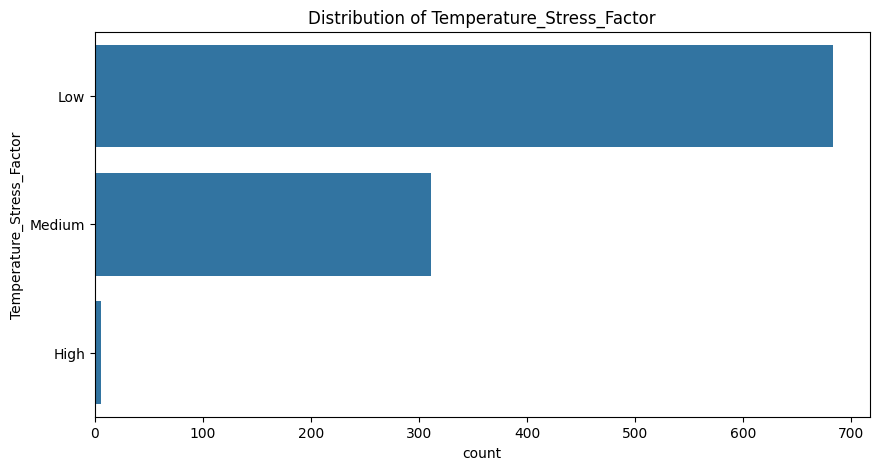
\includegraphics[width=\linewidth]{stress_distr.png}
    \caption{Distributia \texttt{Temperature\_Stress\_Factor}.}
    \label{fig:countplot_stress}
\end{figure}


\textit{Observatii:}
\begin{itemize}[noitemsep, topsep=1pt]
    \item \texttt{Plant\_Message\_Type}: Se observa un usor dezechilibru de clasa, voi folosi class weights pentru antrenarea modelului.
\end{itemize}

\subsection{Analiza Corelatiei intre Atributele Numerice}
\begin{figure}[H]
    \centering
    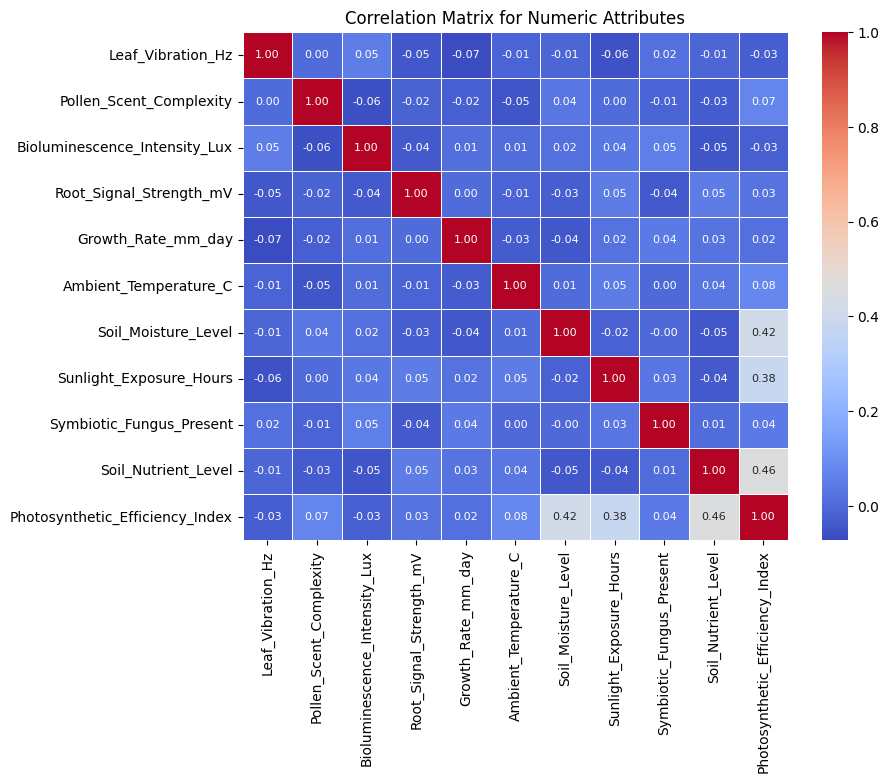
\includegraphics[width=0.8\textwidth]{correlation.png} %
    \caption{Matricea de Corelatie pentru Atributele Numerice.}
    \label{fig:correlation_matrix}
\end{figure}

\textit{Observatii:}
\sloppy
\begin{itemize}[noitemsep, topsep=1pt]
    \item Majoritatea corelatiilor intre variabilele numerice sunt slabe (valori apropiate de 0).
    \item Corelatiile mai notabile, desi moderate, sunt observate intre \texttt{Photosynthetic\_Efficiency\_Index} si \texttt{Soil\_Nutrient\_Level} (0.52), \texttt{Soil\_Moisture\_Level} (0.43), si \texttt{Sunlight\_Exposure\_Hours} (0.39). Aceste corelatii indica logica de generare a indicelui de eficienta.
\end{itemize}

\end{document}